\section{ST-GNN Architecture and Training}
To model the coupled spatial-temporal dynamics of transient fluid flow directly on the native reservoir graph, we implement a Spatio-Temporal Graph Neural Network (ST-GNN). The architecture, illustrated in Fig.~\ref{fig:stgnn_architecture}, couples physical message-passing operations with recurrent temporal state propagation.

\begin{figure}[htbp]
    \centering
    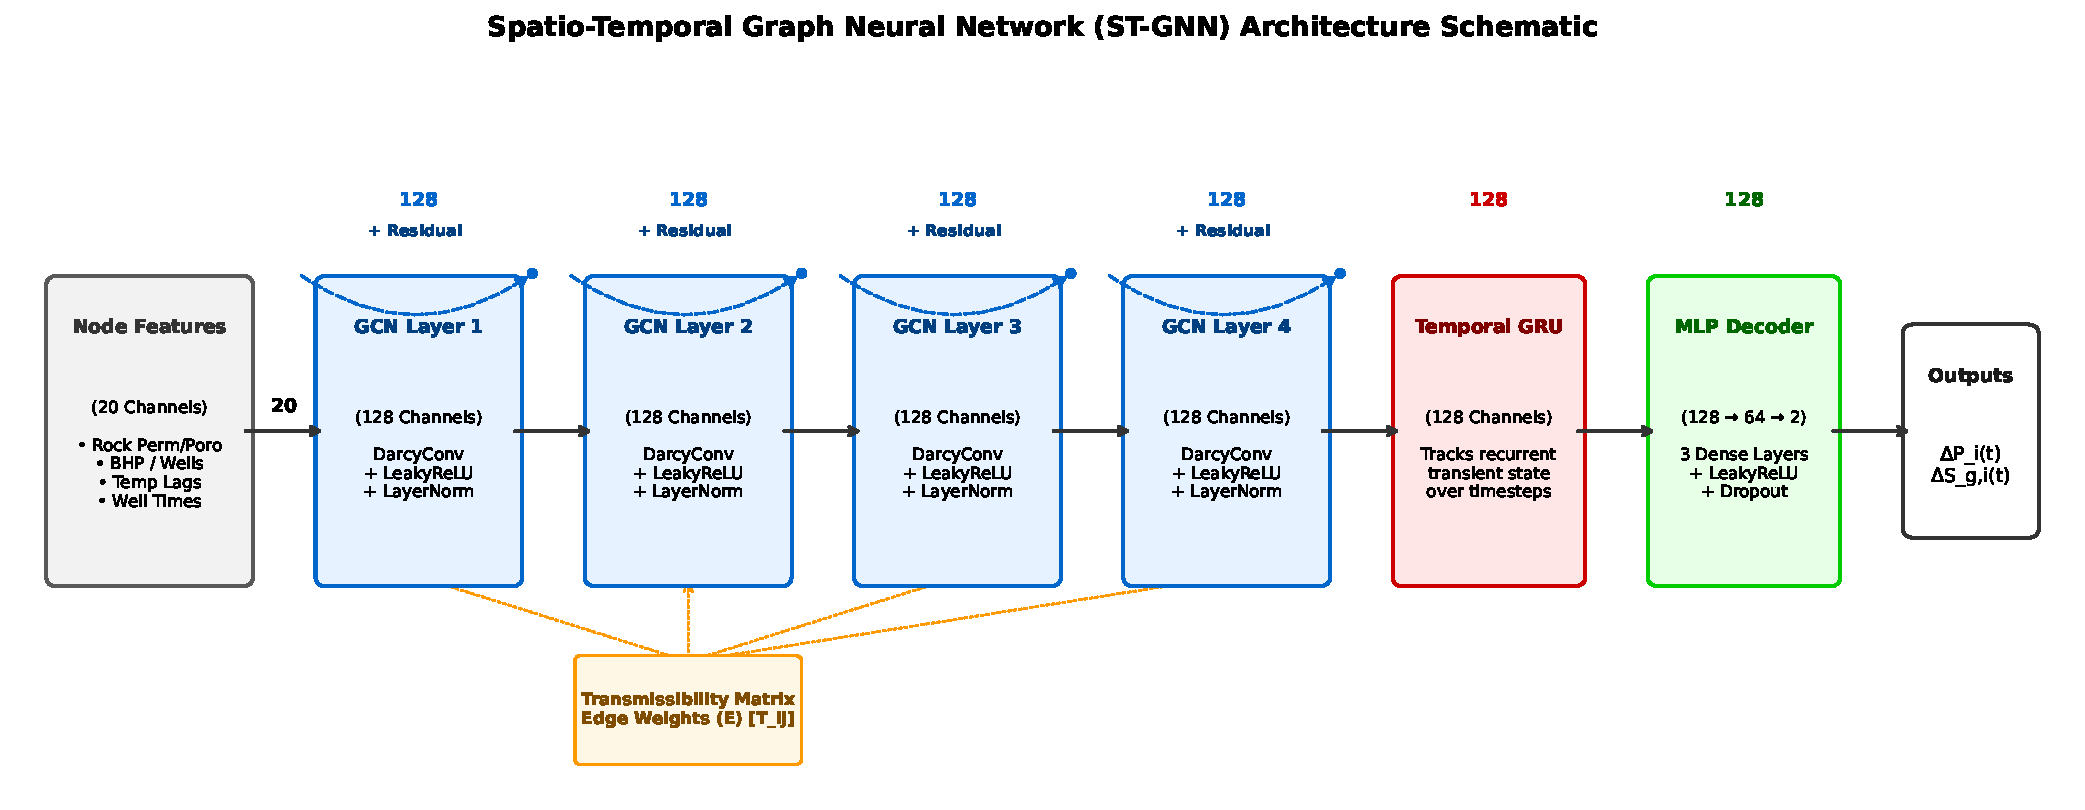
\includegraphics[width=0.95\columnwidth]{figures/fig7_stgnn_architecture}
    \caption{Architecture of the Spatio-Temporal Graph Neural Network (ST-GNN), showing the integration of node/edge inputs, stacked transmissibility-weighted graph convolutions with residual skip connections and LayerNorm, and the GRU block for recurrent temporal update.}
    \label{fig:stgnn_architecture}
\end{figure}

\subsection{Message Passing Formulation}
Fluid transport between face-adjacent cells is modeled using a physical transmissibility-weighted graph convolution layer. The spatial message aggregation at layer $l$ is defined as:
\begin{equation}
\label{eq:mp}
m_{i}^{(l)} = \sum_{j \in N(i)} \tilde{T}_{ij} \text{MLP}_{\text{neigh}} \left( \mathbf{h}_j^{(l-1)} \right) + \text{MLP}_{\text{self}} \left( \mathbf{h}_i^{(l-1)} \right)
\end{equation}
where $\tilde{T}_{ij} = T_{ij} / \sum_{k \in N(i)} T_{ik}$ is the row-normalized inter-cell transmissibility weight, $N(i)$ represents the face-adjacent neighbors of cell $i$, and the $\text{MLP}$ blocks are single linear layers. This formulation directly mimics the Finite Volume discretization in Eq.~\ref{eq:fvm}, with the network learning residual corrections to the transmissibility-weighted Darcy flux. 

To stabilize training through deep stacks and prevent gradient issues, we stack four graph convolutional layers with residual connections, Layer Normalization (LayerNorm), and LeakyReLU activations:
\begin{equation}
\label{eq:residual_gcn}
\mathbf{h}_i^{(l)} = \text{LayerNorm} \left( \text{LeakyReLU}\left( m_i^{(l)} \right) + W_{\text{res}} \mathbf{h}_i^{(l-1)} \right)
\end{equation}
The residual projection weight $W_{\text{res}}$ is a linear mapping used to match hidden dimensions where necessary. Applying LayerNorm after the residual addition stabilizes the node feature variance as it propagates through the graph layers.

\subsection{Temporal Updates and Gated State}
Following spatial aggregation, a Gated Recurrent Unit (GRU) updates the local node hidden states across timesteps, capturing the temporal transient pressure history. The final hidden state $\mathbf{s}_i(t) \in \mathbb{R}^{d_h}$ for each node is passed through a multi-layer perceptron decoder to predict the normalized pressure and gas saturation increments:
\begin{equation}
\label{eq:decoder}
\left[\widehat{\Delta P}_i(t),\, \widehat{\Delta S}_{g,i}(t)\right]^T = \text{MLP}_{\text{dec}} \left( \mathbf{s}_i(t) \right)
\end{equation}

\subsection{Scheduled Sampling Curriculum}
Autoregressive forecasting rollouts are highly vulnerable to error accumulation because models trained under pure teacher forcing (where ground-truth states are consumed at every step) suffer from a covariate shift during inference. To mitigate this distribution mismatch, we adopt a scheduled sampling curriculum:
\begin{itemize}
    \item During training, with probability $p_{\text{rollout}}$ (ramped linearly from $0.0$ to $0.5$ over the training epochs), the model's own predictions from the previous step are fed back as inputs for the next step instead of the ground truth.
    \item To maintain physical consistency, gas saturation predictions are clipped to $[0.0,\, 1.0]$ after each rollout step, and the water saturation is updated via the algebraic closure $S_w = 1.0 - S_g$.
\end{itemize}

\subsection{Multi-Objective Loss Sweep}
Because the surrogate co-emulates pressure and saturation dynamics, the training loss combines normalized Mean Squared Error (MSE) terms for both targets:
\begin{equation}
\label{eq:loss}
\mathcal{L} = \alpha_P \mathcal{L}_P + \alpha_{S_g} \mathcal{L}_{S_g}
\end{equation}
where $\mathcal{L}_P$ and $\mathcal{L}_{S_g}$ are computed in the normalized space to place both targets on comparable scales, and $\alpha_P, \alpha_{S_g}$ are weighting coefficients. To systematically balance pressure and saturation accuracy, we conducted a parameter sweep over three loss-weight configurations:
\begin{enumerate}
    \item \textbf{Balanced}: $\alpha_P : \alpha_{S_g} = 0.5 : 0.5$
    \item \textbf{Pressure-Heavy}: $\alpha_P : \alpha_{S_g} = 0.7 : 0.3$
    \item \textbf{Saturation-Heavy}: $\alpha_P : \alpha_{S_g} = 0.3 : 0.7$
\end{enumerate}

To compare these configurations on a common dimensionless basis, we define a composite balance score:
\begin{equation}
\label{eq:composite_score}
\text{Score} = \frac{\overline{\text{RMSE}}_P}{\bar{P}_{\text{ref}}} + \frac{\overline{\text{RMSE}}_{S_g}}{1.0}
\end{equation}
where $\overline{\text{RMSE}}_P$ is the mean pressure RMSE over the rollout, $\bar{P}_{\text{ref}} = 120.70$~bar is the reference training mean pressure, and $\overline{\text{RMSE}}_{S_g}$ is the mean gas saturation RMSE. The configuration that minimizes this score is selected for rollout evaluation.

Normalization of the constituent errors is mathematically necessary because pressure (measured in bars, spanning $\mathcal{O}(10^2)$) and gas saturation (a dimensionless fraction bounded within $[0.0, 1.0]$) represent completely different physical scales and units. Directly summing their raw RMSEs would cause the pressure error to dominate the metric by several orders of magnitude, rendering joint performance evaluation impossible. Dividing the pressure error by the average operating pressure $\bar{P}_{\text{ref}}$ maps the pressure discrepancy into a dimensionless relative deviation. Equal weighting (a 1:1 ratio) is selected to represent a balanced physical trade-off between the two co-emulated phases. Operationally, pressure dynamics (which govern flow drive and caprock geomechanical stress limits) and gas saturation (which governs hydrogen plume migration and gas-in-place inventory) are of equal importance in underground storage management. The composite score thus provides a single, physically consistent, dimensionless metric for multi-phase tracking quality.
